\documentclass[a4paper]{article}
\usepackage[utf8]{inputenc}
\usepackage[T1]{fontenc}
\usepackage[slovene]{babel}
\usepackage{lmodern}
\usepackage{hyperref}
\usepackage{blindtext}
\usepackage{amssymb}  
\usepackage{listings} %python koda
\usepackage{graphicx}
\usepackage{tabularx}
\usepackage{tikz}
\lstset{%
   breaklines=true
}

\begin{document}

\begin{titlepage}
\center
\textsc{\LARGE Univerza v Ljubljani}\\[0.6cm]
\textsc{\Large Fakulteta za matematiko in fiziko}\\[0.6cm]

{\huge\bfseries Dotikanje največ kvadratov}\\[0.4cm]


\vfill\vfill\vfill

{ Ana Marija Okorn in Sebastjan Šenk}

{ December, 2021}

\vfill

\end{titlepage}

\tableofcontents

\newpage

\section{Uvod}

V  nadaljnih delih poročila bova predstavila problem dotikanja največ kvadratov in kodo, s katero sva ta problem rešila. Na začetku bova opisala najin problem in kakšne cilje sva si zastavila, v nadaljevanju pa bova kodo podrobneje komentirala in predstavila rezultate, do katerih sva prišla.

\section{Naloga}

Given a set of axis-parallel squares in the plane, find a point in the plane that touches as many of the squares as possible. Use ILP to solve this problem. Make experiments generating axis-parallel squares and finding the optimal solution(s). What about finding the line that touches as many squares as possible?

\section{Opis problema}

Podano imamo množico, ki vsebuje enotske kvadrate, katerih stranice morajo biti vzporedne koordinatinm osem in njihova dolžina enaka 1. Te kvadrate bova generirala iz naključno izbranih točk na kordinatni ravnini, kjer bo $x_i \in [x_{\min}, x_{\max}]$  in $y_i \in [y_{\min}, y_{\max}].$Kvadrate bova generirala s pomočjo dolžine stranice. Najprej bova naredila eksperiment z manjšim številom kvadratom, kasneje pa bova pogledala tudi za večje množice kvadratov. S pomočjo celoštevilskega linearnega programiranja (CLP) morava poiskati točko, ki se bo dotikala največ kvadratov. Torej to, kar bova iskala, bo presek največ kvadratov. Pri risanju kvadratov si bova pomagala s knjižnico Matplotlib v Pythonu.  Kasneje pa bova poiskušala poiskati še premico, ki se bo dotikala največ kvadratov. Za to težavo bova za vsako premico $y = kx + m$ , za vsak $k$ in $m$, s pomočjo programa preštela, koliko kvadratov premica seka. Za reševanje obeh CLP programov si bova pomagala s Sage-om in njegovimi vgrajenimi funkcijami za reševanje CLP programov.

\newpage{}

\section{Celoštevilsko linearno programiranje}

Problem bova reševala s pomočjo celoštevilskega linearnega programiranja. Reševanje problemov s CLP je v praksi računsko zelo zahtevno, saj je CLP NP-težek problem, se pravi ne poznamo učinkovitih polinomskih algoritmov za reševanje. Celoštevilski linearni program je definiran na sledeč način. \\
Imamo podatke:
$$A \in \mathbb{R}^{m \times n}, c \in  \mathbb{R}^{n}, b \in  \mathbb{R}^{m }. $$ Iščemo: $$x \in  \mathbb{Z}^{n},$$kjer je doseženo$$maxc^Tx$$
pri pogojih $$Ax\le b\\$$ $$x \ge 0.$$

\section{CLP program za problem največjvečjega dotikanja kvadratov}

\subsection{CLP za iskanje točke, ki se dotika največ kvadratov}

Vhodni podatki:

\begin{itemize}
\item{$n$ \dots število točk, iz katerih zgeneriramo enotske kvadrate} $$n \in \mathbb{N}$$
\item{$x_{i}$ \dots x-koordinata $i$-te točke}
\item{$y_{i}$ \dots y-koordinata $i$-te točke}
\item{$x_{\min} = \min \{x_i \mid 1 \le i \le n\}$}
\item{$x_{\max} = \max \{x_i \mid 1 \le i \le n\}$}
\item{$y_{\min} = \min \{y_i \mid 1 \le i \le n\}$}
\item{$y_{\max} = \max \{y_i \mid 1 \le i \le n\}$}
\end{itemize}

Spremenljivke:

\begin{itemize}
\item{$z_{i}= 1$, če točka $(x,y)$ je v kvadratu $i$}, sicer je $0$, kjer $i \in \{1, 2, \dots, n\}$ in $i \in \mathbb{N}$
\end{itemize}

Iščeva točko $(x,y)$ , za katero velja, da je točka v $i$-tem kvadratu, če veljajo sledeči pogoji:
$$x_i \le x \le x_i+1$$
$$y_i \le y \le y_i+1$$

Iščemo torej \\
$$\max\sum_{i=1}^n z_{i} $$
pri pogojih:
$$z_{i} \in \{0,1\};i \in \{1, 2, \dots, n\}\\$$
$$ x + (1-z_i)(x_{\max} - x_{\min}) >= x_i $$
$$ x - (1-z_i)(x_{\max} - x_{\min}) <= x_i + 1 $$
$$ y + (1-z_i)(y_{\max} - y_{\min}) >= y_i $$
$$ y - (1-z_i)(y_{\max} - y_{\min}) <= y_i + 1 $$

Za začetek si bova problem pogledala v mreži $[0,10]$ x $[0,10]$ pri $n = 60$. Kasneje pa si bova ogledala kako se čas algoritma spreminja z večanjem mreže in z večanjem oz. spreminjanjem števila kvadratov.\\

\subsection{CLP za iskanje premice $y = kx + m,$ ki se dotika največ kvadratov}

Vhodni podatki:

\begin{itemize}
\item{$n$ \dots število točk, iz katerih zgeneriramo enotske kvadrate} $$n \in \mathbb{N}$$
\item{$x_{i}$ \dots x-koordinata $i$-te točke}
\item{$y_{i}$ \dots y-koordinata $i$-te točke}
\item{$x_{\min} = \min \{x_i \mid 1 \le i \le n\}$}
\item{$x_{\max} = \max \{x_i \mid 1 \le i \le n\}$}
\item{$y_{\min} = \min \{y_i \mid 1 \le i \le n\}$}
\item{$y_{\max} = \max \{y_i \mid 1 \le i \le n\}$}
\end{itemize}

Spremenljivke:

\begin{itemize}
\item{$z_{i}= 1$, če premica seka kvadrat $i$}, sicer je $0$, kjer $i \in \{1, 2, \dots, n\}$ in $i \in \mathbb{N}$
\item{$u_{i}= 1$, če premica $y = kx + m$ seka kvadrat $i$}, tako, da je njegovo levo zgornje oglišče nad premico, desno spodnje ogljišče pa pod njo, sicer $u_i$ je $0$, kjer $i \in \{1, 2, \dots, n\}$ in $i \in \mathbb{N}$
\item{$v_{i}= 1$, če premica $y = kx + m$ seka kvadrat $i$},  tako, da je njegovo levo spodnje oglišče pod premico, desno zgornje ogljišče pa nad njo, sicer $v_i$ je $0$, kjer $i \in \{1, 2, \dots, n\}$ in $i \in \mathbb{N}$
\end{itemize}

Pred tem definiramo in izračunamo še $p_{\max} = k (x_{\max}+1)+m$ in $p_{\min} = k (x_{\min})+m,$ ki predstavljata maksimalno in minimalno vrednost izmed vseh možnih $k$ in $m$, ki jih lahko dosežemo. 

Iščemo torej \\
$$\max\sum_{i=1}^n z_{i} $$
pri pogojih:\\
$$z_{i} \in \{0,1\}; i \in \{1, 2, \dots, n\}\\$$
$$z_i <= u_i + v_i$$   
$$k x_i + m - (1 - u_i) (p_{\max} - y_{\min}) <= y_i + 1$$
$$k (x_i+1) + m + (1 - u_i) (y_{\max} - p_{\min}) >= y_i $$
$$k x_i + m + (1 - v_i) (y_{\max} - p_{\min}) >= y_i$$
$$k (x_i+1) + m - (1 - v_i) (p_{\max} - y_{\min}) <= y_i + 1$$

\section{Cilji}

Eden izmed najinih ciljev je s pomočjo celoštevilskega linearnega programiranja pravlino rešiti problem iskanja točke in premice, ki se dotika največ enotskih kvadratov.
Najin cilj je tudi, da ugotoviva, kako se spreminja čas delovanja programa ob spreminjanju:

\begin{itemize}
\item{števila n oziroma ob povečanju števila kvadratov,}
\item{velikosti izbrane mreže.}
\end{itemize}

\section{Koda}

\subsection{Pomožne funkcije}

V nadaljevanju so predstavljene najine kode za reševanje tega problema.  Za zečetek sva si pripravila nekaj funkcij in drugih pripomočkov, za pomoč pri reševanju najnega problema.
\\
Za začetek reševanja problema si je potrebno izbrati začetno delovno okolje. Kot omenjeno sva si za iskanje točke in premice, ki se dotikata največ kvadratov, izbrala, da bova to preverjala za parametre $n = 60, x_{min} = 0, x_{max} = 10, y_{min} = 0, y_{max} = 10.$ Lahko pa si izberemo poljubne parametre.
Za začetek sva naredila funkcijo \texttt{nakljucne\_tocke}, ki nam zgenerira n naključnih točk v mreži $x_i \in [x_{\min}, x_{\max}-1]$  in $y_i \in [y_{\min}, y_{\max}-1]$ s pomočjo vgrajene funkcije random.uniform(). Koda s pomočjo katere sva to generirala je naslednja:

\begin{lstlisting}[language=Python]
def nakljucne_tocke(x_min, x_max, y_min, y_max, n):
    rangeX = (x_min, x_max-1)
    rangeY = (y_min, y_max-1)
    tocke = []
    i = 0
    while i<n:
        x = random.uniform(*rangeX) 
        y = random.uniform(*rangeY)
        tocke.append([x,y])
        i += 1
    return tocke
seznam_tock = nakljucne_tocke(x_min, x_max, y_min, y_max, n)
\end{lstlisting}

Nato sva zgenerirala še ostale tri točke ob tem predpostavljamo, da so prej generirane točke leva spodnja ogljišča enotskih kvadratov. S funkcijo \texttt{koordinate\_kvadrata} sva kot izhodni seznam dobila seznam točk, ki generirajo kvadrat pri izbrani točki. Nato pa sva v prazen seznam imenovan \texttt{seznam\_kvadratov} shranila vse sezname točk, ki v našem primeru generirajo kvadrate.

\begin{lstlisting}[language=Python]
def koordinate_kvadrata(tocka):
    x0 = tocka[0]
    y0 = tocka[1]
    x1 = x0 + 1
    x2 = x1
    x3 = x0
    y1 = y0
    y2 = y0 + 1
    y3 = y2
    return [[x0,y0], [x1,y1], [x2,y2], [x3,y3]]
seznam_kvadratov = []  
for i in seznam_tock:
    seznam_kvadratov.append(koordinate_kvadrata(i))
\end{lstlisting}

Pri reševanju CLP programa za premico bomo potrebovali tudi vrednosti $p_{\max} = k (x_{\max}+1)+m$ in $p_{\min} = k (x_{\min})+m,$ ki predstavljata maksimalno in minimalno vrednost izmed vseh možnih $k$ in $m$, ki jih lahko dosežemo. Za ta namen sva definirala spodnjo funkcijo \texttt{p\_max\_in\_p\_min}, ki vrne kot izhodni podatek $p_{min}$ in $p_{max},$ ki ju potrebujemo kot vhodni podatek poleg \texttt{seznam\_tock} pri reševanju CLP problema za premico.

\begin{lstlisting}[language=Python]
def p_max_in_p_min(x_min, x_max, y_min, y_max):
    oglisca = [(0, 0), (0, 1), (1, 0), (1, 1)]
    seznam = []
    for i, (x_i, y_i) in enumerate(seznam_tock): 
        for x_j, y_j in seznam_tock[i+1:]: 
            for w_i, z_i in oglisca: 
                for w_j, z_j in oglisca: 
                    k = ((y_j+z_j) - (y_i+z_i)) / ((x_j+w_j) - (x_i+w_i))
                    m = y_i+z_i - k * (x_i+w_i)
                    for x in (x_min, x_max+1): 
                        seznam.append(k*x + m)
    p_min = min(seznam)
    p_max = max(seznam)
    return [p_min, p_max]
\end{lstlisting}

\subsection{Koda za CLP }

S pomočjo spodnje kode sva si pomagala rešiti CLP program za iskanje točke in premice. Funkcija \texttt{najvecje\_dotikanje} reši CLP za iskanje točke. Omenjena funkcija vrne kot izhodni podatek seznam, v katerem je največje število kvadratov, ki se jih točka dotika. Na drugem mestu v seznamu sta koordinati točke, ki se dotika največ kvadratov. Funkcija pa vrne tudi seznam indeksov kvadratov. Kvadrat je namreč indeksiran kot $i$-ta točka, iz katere je generiran. Funkcija \texttt{najvecje\_dotikanjepremica} pa nam pomaga rešiti CLP za iskanje premice, ki se dotika največ kvadratov. Le ta vrne enak izhodni podatek kot CLP za točko, le da namesto kordinate točke dobimo vrednost koeficienta $k$ in začetne vrednosti $m$ premice $y = k*x + m$ (to je ta premica, ki jo iščemo).

\begin{lstlisting}[language=Python]
def najvecje_dotikanje(seznam_tock):
    n = len(seznam_tock)
    x_min = min(x for x, y in seznam_tock)
    x_max = max(x for x, y in seznam_tock)
    y_min = min(y for x, y in seznam_tock)
    y_max = max(y for x, y in seznam_tock)

    p = MixedIntegerLinearProgram(maximization=True)
    z = p.new_variable(binary=True) 
    p.set_objective(sum(z[i] for i in range(n))) 
    for i, (x_i, y_i) in enumerate(seznam_tock): 
        p.add_constraint(p['x'] + (1-z[i])*(x_max - x_min) >= x_i)
        p.add_constraint(p['x'] - (1-z[i])*(x_max - x_min) <= x_i + 1)
        p.add_constraint(p['y'] + (1-z[i])*(y_max - y_min) >= y_i)
        p.add_constraint(p['y'] - (1-z[i])*(y_max - y_min) <= y_i + 1)

    stevilo = p.solve()
    x, y = p.get_values(p['x']), p.get_values(p['y'])
    kvadrati = [k for k, v in p.get_values(z).items() if v == 1]
    return [stevilo, (x, y), kvadrati] 

def najvecje_dotikanjepremica(seznam_tock, p_max, p_min): 
    n = len(seznam_tock)
    x_min = min(x for x, y in seznam_tock)
    x_max = max(x for x, y in seznam_tock)
    y_min = min(y for x, y in seznam_tock)
    y_max = max(y for x, y in seznam_tock)
   
    p = MixedIntegerLinearProgram(maximization=True) 
    z = p.new_variable(binary=True) 
    u = p.new_variable(binary=True)
    v = p.new_variable(binary=True)
    p.set_objective(sum(z[i] for i in range(n))) 
    for i, (x_i, y_i) in enumerate(seznam_tock): 
        p.add_constraint(z[i] <= u[i]+v[i])
        p.add_constraint(p['k']*(x_i+1) + p['m'] + (1-u[i])*(y_max - p_min) >= y_i)
        p.add_constraint(p['k']*x_i + p['m'] - (1-u[i])*(p_max - y_min) <= y_i + 1)
        p.add_constraint(p['k']*x_i + p['m'] + (1-v[i])*(y_max - p_min) >= y_i)
        p.add_constraint(p['k']*(x_i+1) + p['m'] - (1-v[i])*(p_max - y_min) <= y_i + 1)
    stevilo = p.solve()
    k, m = p.get_values(p['k']), p.get_values(p['m'])
    kvadrati = [k for k, v in p.get_values(z).items() if v == 1]
    return [stevilo, (k, m), kvadrati] 
\end{lstlisting}

S pomočjo spodnjih dveh ukazov, dobimo rešitev obeh CLP programov.

\begin{lstlisting}[language=Python]
najvecje_dotikanje(seznam_tock)
najvecje_dotikanjepremica(seznam_tock,p_max)
\end{lstlisting}

\subsection{Kode za izvajanje poskusov}

Kot prej omenjeno naju je zanimalo, kako se spreminja čas izvajanja glede na število kvadratov in glede na velikost mreže v koordinatnem sistemu, v katerem smo izbirali točke za generiranje kvadratov. Funkcija \texttt{cas\_izvajanja\_premica} nam pomaga pri opazovanju časov za CLP za premico. Naslednja funkcija pa nama je pomagala pri preučevanju omenjenega pri CLP programu za točko.

\begin{lstlisting}[language=Python]
def cas_izvajanja(x_min, x_max, y_min, y_max ,n):
    seznam_tock = nakljucne_tocke(x_min, x_max, y_min, y_max, n)
    casi = []
    for i in range(1,n+1):
        zacetek = time.time()
        najvecje_dotikanje(seznam_tock)
        konec = time.time() - zacetek
        casi.append((konec))
    return casi
\end{lstlisting}

\begin{lstlisting}[language=Python]
def cas_izvajanja_premica(x_min, x_max, y_min, y_max ,n):
    seznam_tock = nakljucne_tocke(x_min, x_max, y_min, y_max, n)
    p_min = p_max_in_p_min(x_min, x_max, y_min, y_max)[0]
    p_max = p_max_in_p_min(x_min, x_max, y_min, y_max)[1]
    casi = []
    for i in range(1,n+1):
        zacetek = time.time()
        najvecje_dotikanjepremica(seznam_tock,p_max,p_min)
        konec = time.time() - zacetek
        casi.append((konec))
    return casi
\end{lstlisting}

\section{Rezultati za izbran primer}

Kot sva že omenila, sva najin problem dotikanja kvadratov najprej reševala na izbranem problemu s parametri $n = 60, x_{min} = 0, x_{max} = 10, y_{min} = 0, y_{max} = 10.$  Za lažjo nazornost reševanja najinega problema sva si narisala zgenerirane podatke oz. v najinem primeru kvadrate. En primer naključno generiranih kvadratov pri izbranih parametrih je na naslednji sliki.

\begin{figure}[h!]
  \centering
  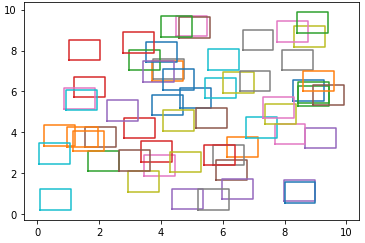
\includegraphics[width= 0.6\textwidth]{kvadrati.png}
  \caption{Primer naključno generiranih kvadratov pri $n = 60, x_{min} = 0, x_{max} = 10, y_{min} = 0, y_{max} = 10.$}
\end{figure}

Funkcija \texttt{najvecje\_dotikanje} reši CLP za iskanje točke in nam vrne $$[5.0, (9.264358087226611, 6.275941115149412), [12, 20, 22, 45, 51]].$$ To nam pove, da se točka $ (9.264358087226611, 6.275941115149412)$ dotika največ kvadratov od vseh točk. Vidimo, da nam program na prvem mestu pove, da se dotika petih kvadratov. Zadnji element seznama, ki ga vrne funkcija je seznam, ki nam pove katere kvadrate se dotika točka. 
Prej definirana funkcija \texttt{najvecje\_dotikanjepremica} pa nam pomaga rešiti CLP za iskanje premice, ki se dotika največ kvadratov in nam vrne v tem primeru $$[18.0, (0.8692548123233682, 1.559674710648847), [0, 2, 8, 10, 13, 15, 18, 19, 28, 31, 36, 39, 40, 41, 42, 44, 47, 49]].$$ Iz tega izvemo, da se poljubna premica v tem primeru dotika največ $18$ kvadratov. Premica, za katero velja, da se dotika največ kvadratov, je $$p = 0.8692548123233682x + 1.559674710648847. $$

\newpage{}

\section{Rezultati poskusov}

Spodnji graf nam prikazuje, kako se povprečno spreminja čas izvajanja CLP programa za iskanje točke, ki se dotika največ kvadratov, v odvisnosti od števila kvadratov. Funkcijo \texttt{najvecje\_dotikanje} sva pognala na mreži $[0,10]$ x $[0,10]$ pri $n \in \{30, 40, \dots, 100\}.$ Iz grafa je razvidno, da se čas izvajanja poveča s povečanjem števila kvadratov, kar je seveda logično, saj mora program za vsak kvadrat preveriti ali je točka v njem ali ne.

\begin{figure}[h!]
  \centering
  \includegraphics[width= 0.6\textwidth]{odvisnost_od_n.png}
  \caption{Graf časa izvajanja CLP-ja za iskanje točke, ki se dotika največ kvadratov, v odvisnosti od števila kvadratov.}
\end{figure}

\newpage{}

Sledeči graf pa nam  prikazuje, kako se povprečno spreminja čas izvajanja CLP programa za iskanje točke, ki se dotika največ kvadratov, v odvisnosti od velikosti mreže, spreminjala pa sva samo spremenljivko $y_{max}$. Časovno zahtevnost sva preverjala za  $x_{min}=0$, $x_{max}=10$,  $y_{min}=0$,  $n=100$, za maksimalno mejo $y$ koordinate pa sva izbrala $y_{max} \in \{10, 20, \dots, 100\} .$ Z razliko od prejšnjega grafa se tukaj časovna zahtevnost ni pretiroma spreminjala glede na velikost opazovane mreže.

\begin{figure}[h!]
  \centering
  \includegraphics[width= 0.6\textwidth]{odvisnost_od_y_max.png}
  \caption{Graf časa izvajanja CLP-ja za iskanje točke, ki se dotika največ kvadratov, v odvisnosti od velikosti mreže oziroma od $y_{max}$.}
\end{figure}

\newpage{}

Spodnji graf nam prikazuje, kako se povprečno spreminja čas izvajanja CLP programa za iskanje premice, ki se dotika največ kvadratov, v odvisnosti od števila kvadratov. Funkcijo \texttt{najvecje\_dotikanjepremica} sva pognala na mreži $[0,10]$ x $[0,10]$ pri $n \in \{10, 20, 30, 40\}.$ Iz grafa je razvidno, da se čas izvajanja kar nekajkrat poveča s povečanjem števila kvadratov. Pri $n=10$ je povprečni čas izvajanja okoli $0,05$ sekunde, pri $n=20$ je čas približno $0,35$ sekunde, medtem ko je pri $n=40$ povprečni čas izvajanja kar $11,85$ sekund, kar je kar $237$-krat počasnejše kot čas izvajanja enega CLP-ja pri $n=10.$ Tu sva opazovala le časovno zahtevnost do $n=40$ saj za $n=50$ program v 8-ih urah ni izračunal teh podatkov, zato sva se odločila, da prekineva in bova prikazala le te podatke, ki so na grafu.
\begin{figure}[h!]
  \centering
  \includegraphics[width= 0.6\textwidth]{odvisnost_od_n_premica.png}
  \caption{Graf časa izvajanja CLP-ja za iskanje premice, ki se dotika največ kvadratov, v odvisnosti od števila kvadratov.}
\end{figure}

\newpage{}

\section{Viri}
\begin{itemize}
\item Arijana Žitnik (2021). Prosojnice Celostevilsko linearno programiranje, časovna zahtevnost in težki problemi. Dostopno na:$https://ucilnica2021.fmf.uni-lj.si/pluginfile.php/58787/mod_resource/content/13/CLP.pdf$
\item Konzultacije z asistentom Janošom Vidalijem in s profesorjem Sergio Cabello.
\end{itemize}

\end{document}